\section{Design Pattern}
Struttura Pattern: nome, problema che risolve, soluzione che propone, conseguenza che porta.

Rendono il codice più comprensibile, flessibile ed'organizzato. Vanno usati dove opportuno. Favorisce rifattorizzazione\footnote{Modifica/Riprogettazione del codice, che non aggiunge funzionalità, per migliorare programmazione/struttura e predisporre a cambiamenti.} nella fase di consolidamento del codice (prototyping, expansionary, consolidating).

Classi di Pattern: Creazionali, Strutturali, Comportamentali.

Scope dei Pattern: relazioni tra Classi (compile-time), relazioni tra Oggetti (run-time).

Principi: DRY (Don't Reapeat Yourself), KISS (Keep It Simple, Stupid), SRP (Single Responsibility Principle), OCP (Open-Closed Principle), DIP (Dependency-Inversion Principle).

\subsection{Strutturali}
\textbf{Proxy (strutturale, Classe)}: Fornisce un oggetto surrogato che controlla l'accesso all'oggetto interessato. Non viene cambiato lo "scopo" ma "pilotato/arricchito".

\begin{center}
	\begin{tikzcd}
		Client \arrow[r, "use", bend left]   & Interface &                                                         \\
		Target \arrow[ru, dashed, bend left] &           & Proxy \arrow[ll, "use"'] \arrow[lu, dashed, bend right]
	\end{tikzcd}
\end{center}

L'oggetto wrapper si compone (ha un campo di tipo interfaccia) dell'oggetto target cosi da gestirne l'uso.
L'oggetto wrapper e target sono interscambiabili, implementando la stessa interfaccia, per il cliente di cui sene compone.

Posso usare più wrapper in cascata.

Separa e incapsula logica d'accesso, target rimane puro. Assicura SRP, OCP, DIP.

\bigskip

\textbf{Decorator (Oggetto)}: Aggiunge responsabilità/funzionalità dinamicamente e flessibilmente ad un'oggetto.

\begin{center}
	\begin{tikzcd}
		Interfaccia                       &  & AbstractDecoratore \arrow[ll, "use" description, bend right] \arrow[ll, dashed, bend left] \\
		Implementazioni \arrow[u, dashed] &  & Decoratori \arrow[u, "estende" description]
	\end{tikzcd}
\end{center}

L'oggetto astratto decoratore si compone (ha un campo di tipo interfaccia) dell'oggetto target cosi da delegare, modificare o aggiungere metodi rispetto all'oggetto targer (implementazioni dell'interfaccia).
L'oggetto astratto decoratore e target sono interscambiabili, implementando la stessa interfaccia.

Posso comporre più decoratori insiemi (decorando un decoratore).

\bigskip

\textbf{Iterator (Oggetto)}: Oggetto per accedere sequenzialmente ad'elementi d'un aggregato (rappresentazione nascosta).

La classe iterabile crea un'iteratore che accede sequenzialemente agli elementi dell'iterabile.

\multiline{}{}{CodiciEsempio/iterator.java}

\bigskip

\textbf{Adapter (Classe/Oggetto)}: Adatta una classe a un'interfaccia richiesta dal'client.

\begin{center}
	\begin{tikzcd}
		Client \arrow[r, "use"] & Interface                                  &        \\
		& Adapter \arrow[r, "use"] \arrow[u, dashed] & Target
	\end{tikzcd}
\end{center}

La nuova classe adapter implementa l'interfaccia richiesta dal client e wrappa per composizione (ha un campo di tipo interfaccia) o ereditarietà la classe target. L'adapter redirige, per delegazione o eredità, le chiamate al target.

L'adapter può essere una inner class della classe target (non necessità di composizione o ereditarietà).

\subsection{Comportamentali}
\textbf{Template Method (Classe)}: Definisce il template (scheletro) di un comportamento lasciando l'indicazione di alcuni aspetti alle sottoclassi.

\begin{center}
	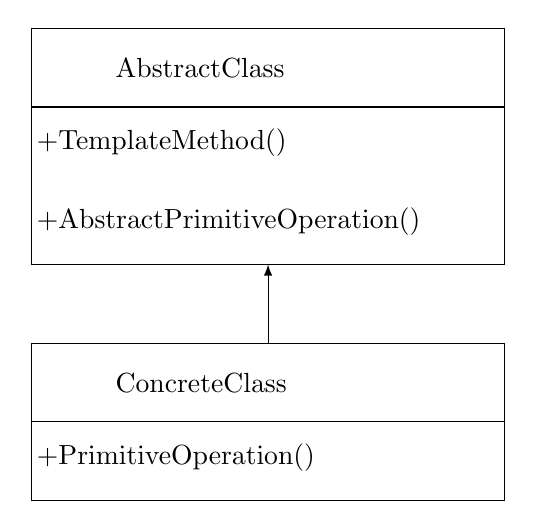
\begin{tikzpicture}
		\node[black, anchor=south west] at (-1.06,1.25) {AbstractClass};
		\node[black, anchor=south west] at (-2.06,0.25) {+TemplateMethod()};
		\node[black, anchor=south west] at (-2.06,-0.75) {+AbstractPrimitiveOperation()};
		\node[black, anchor=south west] at (-2.06,-3.75) {+PrimitiveOperation()};
		\node[black, anchor=south west] at (-1.06,-2.75) {ConcreteClass};
		\draw[draw=black, thin, solid] (-2.00,2.00) rectangle (4.00,-1.00);
		\draw[draw=black, thin, solid] (-2.00,-2.00) rectangle (4.00,-4.00);
		\draw[draw=black, thin, solid] (-2.00,1.00) -- (4.00,1.00);
		\draw[draw=black, thin, solid] (-2.00,-3.00) -- (4.00,-3.00);
		\draw[draw=black, -latex, thin, solid] (1.00,-2.00) -- (1.00,-1.00);
	\end{tikzpicture}
\end{center}

Il comportamento è un metodo non astratto della classe astratta che usa metodi astratti (aspetti implementativi) forniti dalle sotto classi.

Si può attuare anche con interfacce e metodi default.

\bigskip

\textbf{Strategy (Oggetto)}: Definisce un'insieme di comportamenti interscambiabili dai clineti della classe.

\begin{center}
	\begin{tikzcd}
		Client \arrow[r, "use"] & Interface                       \\
		& Comportamenti \arrow[u, dashed]
	\end{tikzcd}
\end{center}

Comportamenti (classi) sono specializzazioni della strategia, l'interfaccia (lambda se interfaccia funzionale) o classe base, di cui si compone (ha un campo di tipo interfaccia) il cliente.

\bigskip

\textbf{Observer (Oggetto)}: Definisce una dipendenza dimanica uno (subject) a molti (listener). Quando l'uno cambia i molti sono notificati e reagiscono.

\begin{center}
	\begin{tikzcd}
		Subject \arrow[rr, "use \ many"] &  & Observer\ (I) &  & Listener \arrow[ll, dashed]
	\end{tikzcd}
\end{center}

L'interfaccia Observer definisce il metodo \inline{update()}, implementato nei listener.
Il subject con \inline{attach()} aggancia i listener di cui si compone (ha un campo di tipo interfaccia) e quando vale una certa condizone chiama con \inline{notilyAll()} l'update su tutti i listener agganciati.




\subsection{Creazionali}
Permenettono il disaccopiamento della creazione degli oggetto dalle classi d'appartenenza.

\bigskip

\textbf{Singleton (Oggetto)}: Garantisce un'unica istanza della classe. Tale istanza è ccessibile globalmente e facilmente ad'altre classi (senza fornire riferimenti).

\begin{center}
	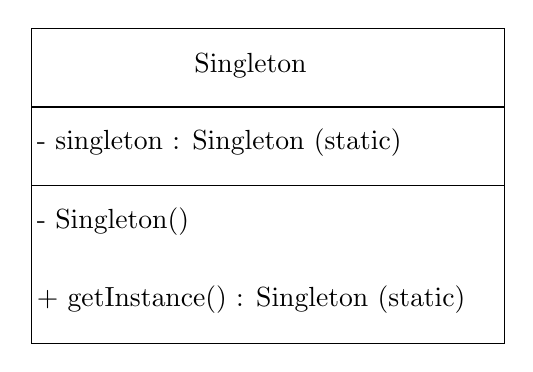
\begin{tikzpicture}
		\draw[draw=black, thin, solid] (-3.00,2.00) rectangle (3.00,-2.00);
		\draw[draw=black, thin, solid] (-3.00,1.00) -- (3.00,1.00);
		\draw[draw=black, thin, solid] (-3.00,0.00) -- (3.00,0.00);
		\node[black, anchor=south west] at (-1.06,1.25) {Singleton};
		\node[black, anchor=south west] at (-3.06,0.25) {- singleton : Singleton (static)};
		\node[black, anchor=south west] at (-3.06,-0.75) {- Singleton()};
		\node[black, anchor=south west] at (-3.06,-1.75) {+ getInstance() : Singleton (static)};
	\end{tikzpicture}
\end{center}

Una classe non istanziabile (costruttore privato) crea internamente l'unica istanza dell'oggetto interessato e fornisce dei metodi statici per interagirci.

\colTwo{Vantaggi: controllo accesso, evità riferimenti, con subclassing si raffina l'implementazione, possibile creazione by-need (lazy)}{Svantaggi: multi-threading, dipendenze nascoste, scelta irreversibile, no SRP (creazione, aspetti interni, limita estendibilità classe)}{45}{45}

Implementazione by-need (thread-safe)? Nel metodo statico get si restituisce l'oggetto costante d'una inner static class. (Le inner static class sono inizializzata al primo utilizzo).

Usare se necessario unica istanza e riferimenti troppo impegnativi.

\bigskip

\textbf{Famiglia D.P. Factory}: Il costruttore deve essere privato.
\begin{itemize}
	\item \textbf{Static Factory}: Classe con metodo statico che genera sua istanza o di sue specializzazioni.

	\item \textbf{Simple Factory}: Classe con metodo non statico che genera instasnza d'un altra calsse Target.

	\item \textbf{Factory Method}: Classe con metodo non statico che genera instanze delle sotto classi dell'interfaccia d'appartenenza.

	\begin{center}
		\begin{tikzcd}
			Creator \arrow[rr, "use", dashed]                      &  & Product                   \\
			ConcreteCreator \arrow[u] \arrow[rr, "create", dashed] &  & ConcreteProduct \arrow[u]
		\end{tikzcd}
	\end{center}

	L'inerfaccia fornisce il metodo \inline{factory()} che crea e restituisce l'oggetto. Gli oggett che implementano l'interfaccia la specializzano definendo la logica di creazione.

	\item \textbf{Abstract Method}: come Factory method ma costruisce più oggetti correlati.
\end{itemize}

